\chapter{VADEMECUM\label{chap:divademecum}}


The DIVADEMECUM is a four-page summary of the commands and the input/output files you have to deal with when using \diva.

\minitoc


\newpage

\vspace*{-3cm}
\section{Scripts and actions}
%\vspace*{-1cm}
\begin{table}[H]
\centering
\caption[DIVADEMECUM: \diva input and output files]{DIVADEMECUM: \diva in- and outputs. When not specified differently, input files are from directory  {\tt ./input} and 
output files are placed in directory {\tt ./output}. Script {\tt divarefe} takes the same inputs as {\tt divacalc}
while {\tt divaanom} and {\tt divasumup} use no other user-provided files than the other scripts. Brackets {\tt [ ]} enclose optional files or parameters. Ex. {\tt [-r]} will replace an input file by the outputs from the scripts.\label{vdm}}

%%\centerline{\shortstack{{\Large{DIVADEMECUM}} \\ {{}} \\ {{}}\\ {{}} \\ {{}}}}

{\scriptsize{
\begin{tabular}{c|c|c}
\toprule
{\Large{Input}} & \shortstack{\Large{{\sf Action}} \\
{\Large{{\tt Execution}}} } & {\Large{ Output}} \\ \midrule
{\tt mycase/input/*}  & 
\shortstack{ 
{  { }  } \\
{\sf load new case} \\
{\tt divaload mycase} } & {\tt ./input/*} \\ \hline
\shortstack{
{\tt topo.dat} \\
{\tt param.par}
}
 & 
\shortstack{
{  { }  } \\
{\sf make gridded topography} \\
{\tt divatopo [-r]  } 
\\
{  { }  }
}
& 
\shortstack{
{\tt TopoInfo.dat} { } [{\tt ./input/TopoInfo.dat}] \\
{\tt topo.grd }  { } [{\tt ./input/topo.grd }]
}
\\ \hline
 \shortstack{
{\tt topo.asc} \\
{\tt topo.gebco} 
}
 & 
\shortstack{
{\sf use dbdb or gebco topography} \\
{\tt dbdb2diva [-r]  } 
\\
{\tt gebco2diva [-r]  } 
}
& 
\shortstack{
{\tt TopoInfo.dat} { } [{\tt ./input/TopoInfo.dat}] \\
{\tt topo.grd }  { } [{\tt ./input/topo.grd }]
}
 \\ \hline
 \shortstack{
{\tt TopoInfo.dat} \\
{\tt topo.grd} \\
{\tt [contour.depth] }
}
 & 
\shortstack{
{\sf make contours} \\
{\tt divacont [-r]  } 
\\
{  { }  }
}
& 
\shortstack{
{  { }  } \\
{\tt coast.cont.*}  { } [{\tt ./input/coast.cont.*}] \\
{  { }  }
}
 \\ \hline
 \shortstack{
 {  { }  } \\
{\tt param.par} \\
{\tt coast.coa} 
}
 & 
\shortstack{
{\sf use ODV contours} \\
{\tt divacoa2cont [-r]  } 
\\
{  { }  }
}
& 
\shortstack{
{  { }  } \\
{\tt coast.cont}  { } [{\tt ./input/coast.cont}] \\
{  { }  }
}
 \\ \hline
 \shortstack{
{\tt param.par} \\
{\tt coast.cont} 
}
 & 
\shortstack{
{\sf check hand-made contours} \\
{\tt divacck [-r] [-v]  } 
\\
{  { }  }
}
& 
\shortstack{
{  { }  } \\
{\tt coast.cont.checked}  { } [{\tt ./input/coast.cont}] \\
{  { }  }
}
 \\ \hline
 ../*/fort.*
 & 
 \shortstack{
 {\sf clean up directories} \\
{\tt divaclean  } 
}
& 
 { }
 \\ \hline
 \shortstack{
{\tt data.dat} \\
{\tt coast.cont} \\
{\tt [./output/fieldatdatapoint.anl]} 
}
 & 
\shortstack{
{\sf eliminate useless data} \\
{\tt divadataclean  [f$_{\min}$  f$_{\max}$]  } 
\\
{  { }  }
}
& 
\shortstack{
{  { }  } \\
{\tt ./input/data.dat} \\
{  { }  }
}
 \\ \hline
 \shortstack{
{\tt data.dat} \\
{\tt coast.cont} \\
{\tt [./output/fieldgher.anl]} 
}
 & 
\shortstack{
{\sf bins of data coverage} \\
{\tt divadatacoverage  [-n] [-r]  } 
\\
{  { }  }
}
& 
\shortstack{
{  { }  } \\
{\tt DATABINS*.dat} \\
{  {\tt RL*.dat }  }
}
 \\ \hline
 \shortstack{
 {  { }  } \\
{\tt param.par} \\
{\tt data.dat} \\
{  { }  } 
}
 & 
\shortstack{
{\sf estimate L and S/N} \\
{\tt divafit [n] [-r]  } 
\\
{  { }  } \\
{  { }  }
}
& 
\shortstack{
{\tt covariance.dat} \\
{\tt covariancefit.dat} \\
{\tt paramfit.dat} \\
{\tt param.par.fit} {  { }  } [{\tt ./input/param.par}]
}
\\ \hline
 \shortstack{
 {  { }  } \\
{\tt param.par} \\
{\tt coast.cont} \\
{ [{\tt coast.cont.dens}]  } 
}
 & 
\shortstack{
{\sf make FE mesh} \\
{\tt divamesh    } 
\\
{  { }  }
}
& 
\shortstack{
{  { }  } \\
{\tt divamesh outputs} \\
{  { }  } 
} 
\\ \hline
 \shortstack{
 {\tt gcvsampling.dat} \\
 {\tt param.par} \\
 {\tt data.dat} \\
 {\tt divamesh outputs} \\
 {[{\tt Uvel.dat,Vvel.dat}} \\
 { $\quad ${\tt UVinfo.dat, constraint.dat}]} \\
 {[{\tt RL.dat, RLinfo.dat}]} 
 }
 & 
\shortstack{
{  { }  } \\
{\sf optimise S/N by cross-validation} \\
{\tt divacv [-r]   } \\
{\tt divacvrand ns nt [-r] }  \\
{\tt divagcv [-r]   } \\
{  { }  } \\
{  { }  }
}
& 
\shortstack{
{  { }  } \\
{  { }  } \\
{\tt gcv.dat} \\
{\tt gcvsnvar.dat} \\
{\tt gcvval.dat} \\
{\tt param.par.gcv} {[{\tt ./input/param.par}] } \\
{  { }  } 
} 
\\ \hline
 \shortstack{
 {  { }  } \\
 {\tt param.par} \\
 {\tt data.dat} \\
 {\tt divamesh outputs} \\
 {[{\tt Uvel.dat,Vvel.dat}} \\
 { $\quad ${\tt UVinfo.dat, constraint.dat}]} \\
 {[{\tt RL.dat, RLinfo.dat}]} \\
 {[{\tt valatxy.coord}] }
}
 & 
\shortstack{
{  { }  } \\
{\sf make analysis} \\
{  { }  } \\
{\tt divacalc    } 
\\
{  { }  } \\
{  { }  } \\
{  { }  }
}
& 
\shortstack{
{  { }  } \\
{\tt GridInfo.dat} \\
{\tt field*.anl} \\
{\tt error*.anl} \\
{\tt *.nc} \\
{  { }  } \\
{[{\tt valatxyascii.anl}]}
} 
\\ \hline
 \shortstack{
 {  { }  } \\
 {\tt param.par} \\
 {\tt data.dat} \\
 {\tt ./output/meshvisu/*} \\
 {[{\tt Uvel.dat,Vvel.dat}} \\
 { $\quad ${\tt UVinfo.dat, constraint.dat}]} \\
 {[{\tt RL.dat, RLinfo.dat}]} 
}
 & 
\shortstack{
{  { }  } \\
{\sf perform full quality control} \\
{\tt divaqc    } 
\\
{  { }  } \\
{  { }  } \\
{  { }  }
}
& 
\shortstack{
{  { }  } \\
{  { }  } \\
{{\tt outliers.dat}} \\
{{\tt outliers.normalized.dat}} \\
{  { }  } \\
{  { }  } 
} 
\\ \hline
 \shortstack{
 {\tt param.par} \\
 {\tt data.dat} \\
{\tt divacalc outputs}
}
 & 
\shortstack{
{  { }  } \\
{\sf perform simple quality control} \\
{\tt divaqcbis } 
\\
{  { }  } \\
{  { }  } \\
{  { }  }
}
& 
\shortstack{
{  { }  } \\
{  { }  } \\
{  { }  } \\
{{\tt outliersbis.dat}} \\
{{\tt outliersbis.normalized.dat}} \\
{  { }  } \\
{  { }  } 
} 
\\ \hline
 \shortstack{
 {\tt param.par} \\
 {\tt data.dat} \\
{\tt divacalc outputs}
}
 & 
\shortstack{
{  { }  } \\
{\sf perform simple quality control} \\
{\tt divaqcter } 
\\
{  { }  } \\
{  { }  } \\
{  { }  }
}
& 
\shortstack{
{  { }  } \\
{  { }  } \\
{  { }  } \\
{{\tt outlierster.dat}} \\
{{\tt outlierster.normalized.dat}} \\
{  { }  } \\
{  { }  } 
} \\ \hline
{\tt ./output/*}  & 
\shortstack{
{\sf make some plots} \\
{\tt divagnu [f$_{\min}$ f$_{\max}$] } 
} & {\tt ./gnuwork/plots/*} \\ \hline
{\tt ./output/*}  & 
\shortstack{
{\sf save results} \\
{\tt divasave mycase} 
}
& {\tt mycase/outut/*} \\ 
\bottomrule
\end{tabular}
}}
\end{table}


%\pagebreak
%\clearpage
%\pagebreak

\section{Workflow}

%%\LaTeXPiX{./figures/images/divademecum}{Scripts used in the command-line version of DIVA; optional arguments are between {\tt []}.}{vade}

\begin{figure}[H]
\centering
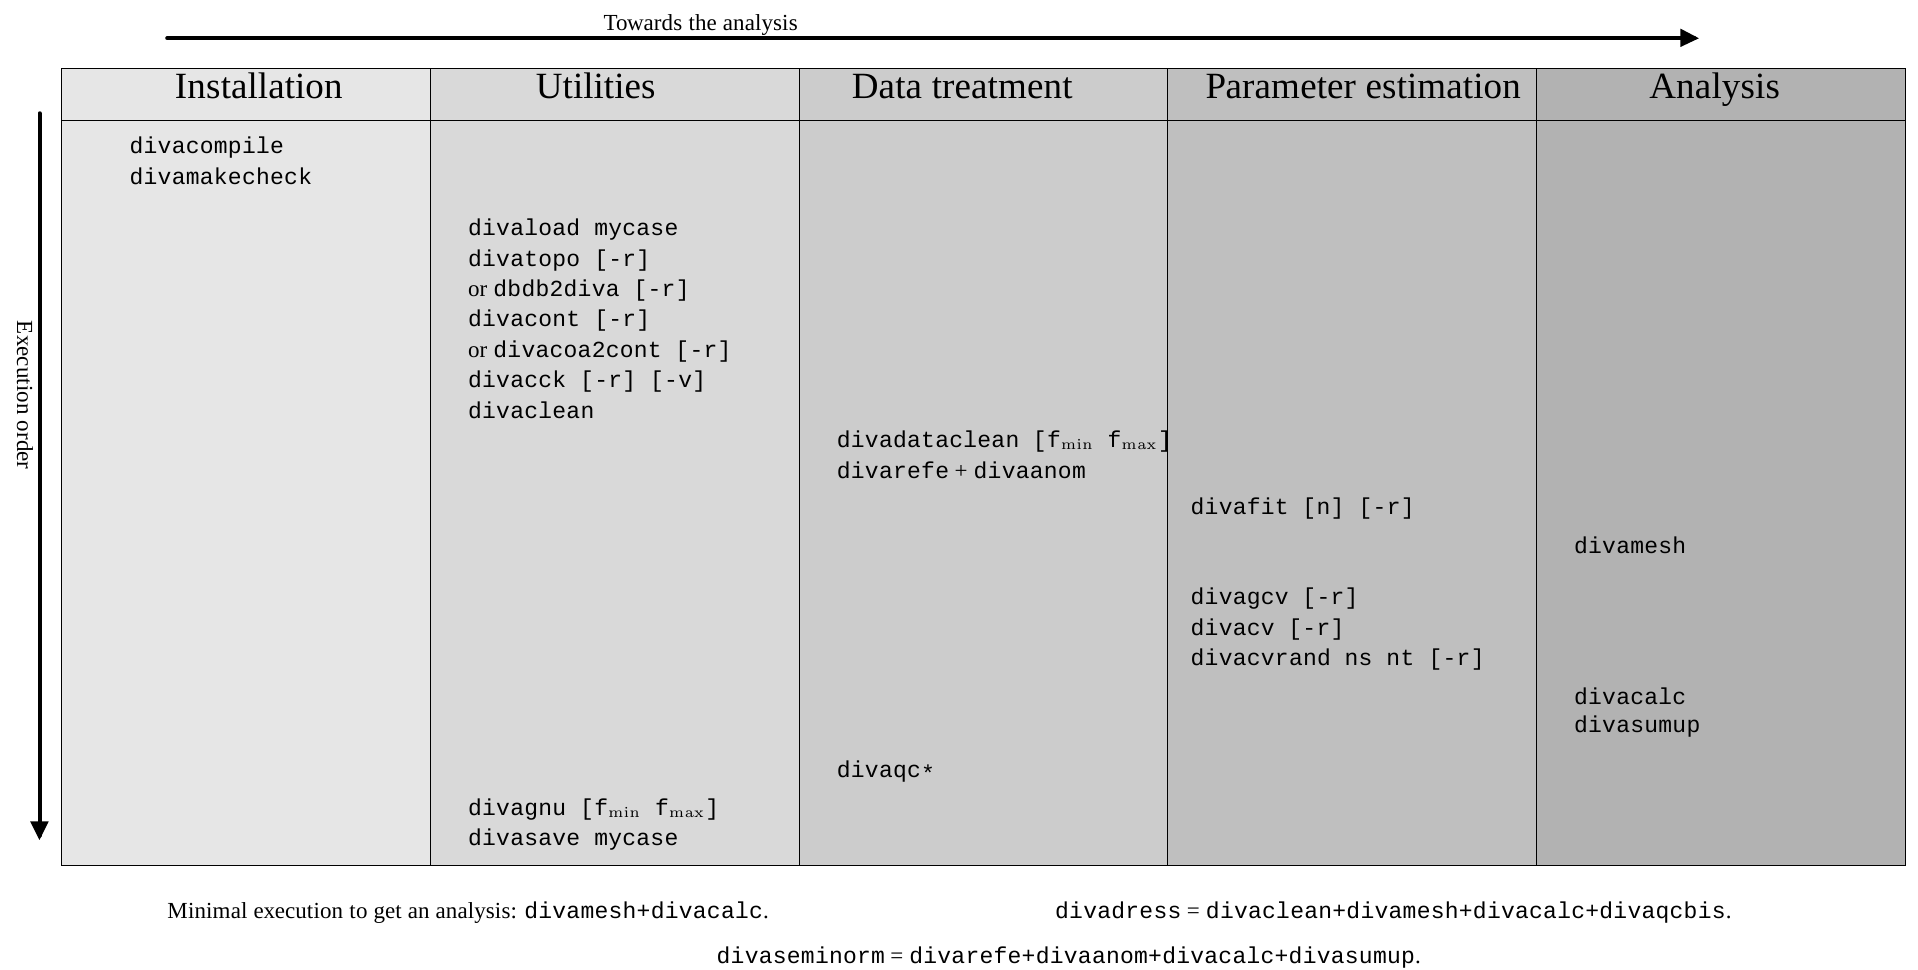
\includegraphics[width=1.25\textwidth,angle=90]{divademecum}
\caption[Scripts used in the command-line version of \diva.]{Scripts used in the command-line version of \diva; optional arguments are between {\tt []}.}
\end{figure}

%\pagebreak
%\clearpage

%\thispagestyle{empty}
%{\Huge{Input files}}
%\vspace*{-3cm}


\section{Input files}
\begin{multicols}{2}
{
\begin{minipage}{.5\textwidth}
\rule{\textwidth}{10pt}
%\begin{figure}
{\tiny{
\begin{verbatim}
# Correlation length (in units of data, if degrees: S-N)
1
# icoordchange (-xscale, 0=none, 1=degtokm, 2=sin projection)
0
# ispec (error output files required)
7
# ireg (subtraction of reference field 0: no, 1:mean, 2:plane)
0
# xori (origin of output regular grid, min values of x)
-4.999
# yori (origin of output regular grid, min values of y)
-4.999
# dx (x-step of output grid)
0.1999
# dy (y-step of output grid)
0.1999
# nx number of x points of output grid
51
# ny number of y points of output grid
51
# valex (exclusion value)
-9999.0
# snr signal to noise ratio 
10
# varbak variance of the background field
1\end{verbatim}
}}
%\hrule{\textwidth}
\vspace*{-0.5cm}
\makebox[\textwidth]{\hrulefill}
{\file{param.par} file content. Parameters are self-explaining, except for error output specification. {\tt ispec=0} means no error field requested; add $+1$ for a gridded error field, $+2$ for error at data location and $+4$ for error at coordinates defined in \file{valatxy.coord}.
From there if you want \begin{itemize}
\footnotesize
\item error based on real covariance:\\ {\tt ispec} $\leftarrow$ {\tt -ispec}
\item error based on real covariance with boundary effect: {\tt ispec} $\leftarrow$ {\tt -ispec-10}
\item poor man's error estimate (quick and underestimated error field): {\tt ispec} $\leftarrow$ {\tt ispec+10}
\end{itemize}
\footnotesize{(ex: {\tt ispec=12} makes a poor man's error estimate at data locations) }}
\end{minipage}
}

\begin{minipage}{.5\textwidth}
\rule{\textwidth}{10pt}
%\begin{figure}
{\scriptsize{
\begin{verbatim}
-5  22 34.8
-2  19 36.1
...
\end{verbatim}
}}
\vspace*{-0.5cm}
\makebox[\textwidth]{\hrulefill}
{\file{data.dat} file content. Simple ascii file with {\tt x,y,val} and optional fourth column containing the relative weight on the data (large value = high confidence)}.\\
\file{topo.dat} is just a special case where the third column represents depth (positive for sea values).
\end{minipage}

%\vfill

\begin{minipage}{.5\textwidth}
\rule{\textwidth}{10pt}
%\begin{figure}
{\scriptsize{
\begin{verbatim}
100 10
\end{verbatim}
}}
\vspace*{-0.5cm}
\makebox[\textwidth]{\hrulefill}

{\file{constraint.dat} file content. \\
First value = weight on advection constraint,\\
second value=diffusion coefficient in advection/diffusion equation.}
\end{minipage}

\begin{minipage}{.5\textwidth}
%\makebox[\textwidth]{\hrulefill}
\rule{\textwidth}{10pt}
%\begin{figure}
{\scriptsize{
\begin{verbatim}
0.01
0.03
0.1
0.3
1
3
10
30
100
\end{verbatim}
}}
\vspace*{-0.5cm}
\makebox[\textwidth]{\hrulefill}
{\file{gcvsampling.dat} file content. A list of trial values for the signal-to-noise ratio used in cross validation tools.}
\end{minipage}

\begin{minipage}{.5\textwidth}
%\makebox[\textwidth]{\hrulefill}
\rule{\textwidth}{10pt}
%\begin{figure}
{\scriptsize{
\begin{verbatim}
1000
750
500
400
300
200
100
0
\end{verbatim}
}}
\vspace*{-0.5cm}
\makebox[\textwidth]{\hrulefill}
{\file{contour.depth} file content with depths for contours and subsequent analysis.}
\end{minipage}

\begin{minipage}{.5\textwidth}
%\makebox[\textwidth]{\hrulefill}
\rule{\textwidth}{10pt}
%\begin{figure}
{\scriptsize{
\begin{verbatim}
0
10
0.1
0.2
101
51
\end{verbatim}
}}
\vspace*{-0.5cm}
\makebox[\textwidth]{\hrulefill}
{\file{*info.dat} file describing the gridding parameters of binary gridded files such as \file{Uvel.dat}, \file{topo.grd}, \file{RL.dat},  \file{fieldgher.anl}, \file{errorfieldgher.anl}. Here first grid point in $(0,10)$, with steps $(0.1,0.2)$ and $101 \times 51$ grid points. Look at examples how to read/write binary files with Fortran or Matlab}
\end{minipage}

\end{multicols}

%\pagebreak
%\clearpage
%%{\Huge{Output files}}

\section{Output files}
\begin{multicols}{2}

%\thispagestyle{empty}


\begin{minipage}{.5\textwidth}
%\makebox[\textwidth]{\hrulefill}
\rule{\textwidth}{10pt}
%\begin{figure}
{\tiny{
\begin{verbatim}
 0.50E+01 1131 0.16E+02 0.43E+02 0.38E+02 0.37E+02 0.13E+00
 ...
 
  flag    ident   x   y   dataval  analysis expected-misfit
\end{verbatim}
}}
\makebox[\textwidth]{\hrulefill}
{\file{outliers*.dat} Sorted outliers, from most suspect to least suspect. Column 1: outlier indicator (larger than 3 suspect), following columns: data identifier, x and y coordinates, original data value, analysed data value, expected misfit.}
\end{minipage}

\begin{minipage}{.5\textwidth}
%\makebox[\textwidth]{\hrulefill}
\rule{\textwidth}{10pt}
%\begin{figure}
{\tiny{
\begin{verbatim}
Correlation length (in degrees latitude)
  3.69890785
 Signal to noise ratio
  0.902823746
 VARBAK
  16.7839489
 For information: correlation length in km is  412.962524
\end{verbatim}
}}
\makebox[\textwidth]{\hrulefill}
{\file{paramfit.dat} Self explaining output from {\tt divafit}. When option {\tt [-r]} is used with {\tt divafit}, an adapted \file{param.par} will be placed in {\tt ./input}.}
\end{minipage}

\begin{minipage}{.5\textwidth}
%\makebox[\textwidth]{\hrulefill}
\rule{\textwidth}{10pt}
%\begin{figure}
{\scriptsize{
\begin{verbatim}
 S/N
  1.99764168
 VARBAK
  1.14215052
\end{verbatim}
}}
\makebox[\textwidth]{\hrulefill}
{\file{gcvsnvar.dat} Self explaining output from {\tt divacv, divagc, divacvrand}. When option {\tt [-r]} is used with cross validation, an adapted \file{param.par} will be placed in {\tt ./input}}.
\end{minipage}

\end{multicols}
